\documentclass[journal, a4paper]{IEEEtran} %onecolumn, draftcls
\usepackage{skieeetrans}

% TikZ libraries
\usetikzlibrary{shapes,
shapes.geometric, 
arrows.meta,
intersections, 
positioning, 
dsp, 
chains,
decorations.pathreplacing,
scopes,
fadings,
calc,
matrix,
fit,
quotes
}

\begin{document}
\title{A Compressive Sensing Codec Architecture for ECG Signals
with Adaptive Quantization and Stream Entropy Coding}


\author{Shailesh~Kumar,
        Surendra~Prasad,~\IEEEmembership{Senior Member,~IEEE,}
        and~Brejesh~Lall,~\IEEEmembership{Member,~IEEE}% <-this % stops a space
}

% make the title area
\maketitle
%!TEX root = paper_ecg_cs_codec.tex
% As a general rule, do not put math, special symbols or citations
% in the abstract or keywords.
\begin{abstract}
Remote monitoring of electrocardiogram (ECG) signals
plays a critical role in the management of cardiovascular
diseases. Current long term ECG monitoring systems
generate a large amount of data that need to be
sent across a wireless body area network.
The wearable devices are resource limited.
Hence a low resource consuming compression
scheme is desirable.
Compressive sensing (CS) is quite appealing
as a low complexity method for compression of
ECG data. This paper investigates the distribution
of the compressive measurements and proposes
a CS based codec architecture comprising
simple quantization and
asymmetric numeral systems (ANS) based
entropy coding steps
that can significantly boost the compression ratio
without sacrificing reconstruction performance.
The encoder has low computational complexity
beyond the sensing operation
and can be implemented entirely using integer arithmetic.
The quantized Gaussian entropy model for the compressive measurements
is estimated directly from the data and can be easily adapted
to achieve better compression. Our decoder architecture
is flexible in choosing any suitable reconstruction method.
We have tested our encoder with bound optimization
based block sparse Bayesian learning (BSBL-BO)
reconstruction algorithm on MIT-BIH Arrhythmia database.
We have validated that our encoder can achieve
additional 20-30\% of space savings without any
impact on reconstruction quality on top of the
savings in terms of measurements. We have
also clearly described the digitization process
for the measurements which has often been ignored
in the literature on CS based compression of ECG data. 
As part of reproducible research we have open sourced
our codec (implemented in Python with JAX based GPU
acceleration for the decoder).
\end{abstract}


\IEEEpeerreviewmaketitle

%!TEX root = paper_ecg_cs_codec.tex
\section{Introduction}
\label{sec:intro}
In wireless body area networks (WBAN)
based telemonitoring networks\cite{cao2009enabling},
the energy consumption on sensor nodes is
a primary design constraint \cite{milenkovic2006wireless}.
The wearable sensor nodes are often battery-operated.
It is necessary to reduce energy consumption as
much as possible.
It is desirable that a low-complexity encoder
is used for the compression of ECG data from wearable
devices.
Compressive sensing (CS) \cite{donoho2006compressed,baraniuk2007compressive,
candes2006compressive, candes2008introduction, candes2006near}
provides a very good solution to implement low-complexity encoders
and has been extensively studied for ECG data
compression \cite{craven2014compressed,kumar2022review}.
It uses a sub-Nyquist sampling method by acquiring a small number
of incoherent measurements which are sufficient to reconstruct
the signal if the signal is sufficiently sparse in some
basis.
For a sparse signal $\bx \in \RR^n$, one would make
$m$ linear measurements where $m \ll n$ which can be
mathematically represented by a sensing operation
\begin{equation}
\by = \Phi \bx
\end{equation}
where $\Phi \in \RR^{m \times n}$ is a matrix
representation of the sensing process and $\by \in \RR^m$
the set of $m$ measurements collected for $\bx$.
A suitable reconstruction algorithm can recover $\bx$
from $\by$.

Ideally, the sensing process should be implemented at the
hardware level in the analog-to-digital conversion (ADC) process.
However, much of the use of CS in ECG follows
a digital CS paradigm \cite{mamaghanian2011compressed} where
the ECG samples are acquired first by the ADC circuit on the
device and then they are translated into incoherent
measurements via the multiplication of a digital sensing matrix.
These measurements are then transmitted
to remote telemonitoring servers.
A suitable reconstruction algorithm is used on the server
to recover the original ECG signal from the compressive measurements.
Reconstruction algorithms for ECG signals include:
greedy algorithms 
\cite{polania2011compressed} (simultaneous orthogonal matching pursuit),
optimization-based algorithms \cite{zhang2014energy},
\cite{mamaghanian2011compressed} (SPG-L1),
Bayesian learning algorithms
\cite{zhang2012compressed,zhang2014spatiotemporal,zhang2013extension},
and deep learning based algorithms \cite{zhang2021csnet}.

We consider the problem of efficient transmission of
compressive measurements of ECG signals over the wireless body
area networks under the digital compressive sensing paradigm.
Let $\bx$ be an ECG signal and $\by$ be the corresponding
stream of compressive measurements. Our goal is to
transform $\by$ into a bitstream $\bs$ with as few bits
as possible without losing the signal reconstruction quality.
A primary constraint in our design is that the encoder
should avoid any floating point arithmetic.


\subsection{Related Work}

The literature on the use of CS for ECG compression is mostly
focused on the design of a specific \emph{sensing matrix},
\emph{sparsifying dictionary}, or \emph{reconstruction algorithm}
for the high-quality reconstruction of the ECG signal from the
compressive measurements.
To the best of our knowledge, (digital) quantization and entropy coding of
the compressive measurements of ECG data haven't received much attention
in the literature.

Mamaghanian et al.\cite{mamaghanian2011compressed} use a Huffman codebook
which is deployed inside the sensor device. They don't
employ any quantization of the measurements.
The codebook is fixed. It cannot adapt to differing signal
statistics.
Simulation-based studies generally send the floating point compressive
measurements to their decoder modules.
They don't consider the issue of
the number of bits required to encode each measurement.
The compression ratio is often defined simply as $\frac{m}{n}$
or some variant of it
\footnote{Other variants include
$\frac{n}{m}$ \cite{zhang2012compressed},
$\frac{n-m}{n} \times 100$ \cite{zhang2021csnet}}.
The underlying assumption is that the measurements are
encoded using the same number of bits as the original digital samples.
Huffman codes have frequently been used in ECG data
compression for non-CS methods \cite{luo2014dynamic,chouakri2013wavelet}
for entropy coding.
However, entropy coding of CS measurements has largely been ignored.

Asymmetric Numeral Systems (ANS) \cite{duda2013asymmetric}
based entropy coding schemes have seen much success
in recent years for lossless data compression.
They provide superior compression compared to Huffman
like symbol codes.
To the best of our knowledge, ANS stream codes
have not been considered in the past for the entropy
coding of compressive measurements.


\subsection{Contributions}
In this paper, we present an adaptive quantization and
entropy coding scheme for digital compressive measurements.
The adaptive quantization scheme has been designed
to guarantee a norm-bounded quantization noise.
A quantized Gaussian probability model of the measurements
is estimated directly from the data
and the parameters for this model are used
for the entropy coding of the measurements.  
Asymmetric numeral systems (ANS) based
entropy coding is then used for efficient entropy coding
of the quantized and clipped measurements.
Our encoding scheme doesn't require a fixed codebook
for entropy coding.
The encoder can be implemented entirely using integer arithmetic.
% Our implementation is available as part of
% reproducible research on GitHub \cite{kumar2022ecgcodec}.

\subsection{Paper Organization}
The rest of the paper is organized as follows.
\Cref{sec:arch} describes our proposed codec architecture.
\Cref{sec:data} describes the ECG database
used for the evaluation of the codec and the
performance metrics.
The analysis of the experimental results is covered in \cref{sec:results}.
\Cref{sec:conclusion} summarizes our contributions and major findings.


%!TEX root = paper_ecg_cs_codec.tex
\section{ECG Database and Performance Metrics}
\label{sec:data}

We use the MIT-BIH Arrhythmia Database \cite{moody2001impact}
from PhysioNet \cite{goldberger2000physiobank}.
The database contains 48 half hour excerpts of two channel
ambulatory ECG recordings from 47 subjects.
The recordings were digitized at 360 samples per second
for both channels with 11 bit resolution over a 10mV range.
The samples can be read in both digital (integer) form or
as physical values (floating point) via the software provided
by PhysioNet.
We use the integer values in our experiments since our
encoder is designed for integer arithmetic.
We use the MLII signal (first channel)
from each recording in our experiments.

\subsection{Performance Metrics}
\label{sec:codec:metrics}
In our encoder, ECG signal is split into windows
of $n$ samples each which can be multiplied
with a sensing matrix. Each window of $n$
samples generates $m$ measurements by the
sensing equation $\by = \Phi \bx$.
Assume that we are encoding $s$ ECG samples where
$s = n w$ and $w$ is the number of signal windows
being encoded.
Let the ECG signal be sampled by the ADC device
at a resolution of $r$ bits per sample
\footnote{For MIT-BIH Arrhythmia database, $r=11$.}.
Then the number of uncompressed bits is given by
$\bits_u = r s$.

\subsubsection{Compression Ratio}
Let the total number of compressed
bits corresponding to the $s$ ECG samples be
$\bits_c$ \footnote{This includes the overhead bits required
for the stream header and frame headers to be explained later.}.
Then the \emph{compression ratio} ($\compr$) is defined as
\begin{equation}
\compr \triangleq \frac{\bits_u}{\bits_c}.
\end{equation}
\emph{Percentage space saving} ($\pss$) is defined as
\begin{equation}
\pss \triangleq \frac{\bits_u - \bits_c}{\bits_u} \times 100.
\end{equation}
Note that often in literature, $\pss$ is defined as compression ratio
(e.g., \cite{mamaghanian2011compressed}).
Several papers ignore the bitstream formation aspect
and report $\frac{m}{n} \times 100$
(e.g., \cite{zhang2016comparison})
or $\frac{n - m}{n} \times 100$ (e.g., \cite{zhang2021csnet})
as the compression ratio
which measures the reduction in number of measurements
compared to the number of samples in each window.
We shall call this metric as \emph{percentage measurement
saving} ($\pms$):
\begin{equation}
\pms \triangleq \frac{n - m}{n} \times 100.
\end{equation}
The ratio $m/n$ will be called as the \emph{measurement ratio}:
\begin{equation}
\mathrm{MR}= \frac{m}{n}.
\end{equation}

The measurement ratio $\frac{m}{n}$ is not a
good indicator of compression ratio.
If the sensing matrix $\Phi$ is Gaussian,
then the measurement values are real valued.
In literature using Gaussian sensing matrices
(e.g., \cite{zhang2016comparison}),
it is unclear how many bits are
being used to represent each floating point measurement value
for transmission.
Under standard 32-bit IEEE floating point format,
each value would require 32-bits.
Then for MIT-BIH data the compression ratio in bits
would be $\frac{11 \times n}{32 \times m}$.
The only way the ratio $\frac{m}{n}$ would make sense
if the measurements are also quantized at 11 bits
resolution. However the impact of such quantization
is not considered in the simulations.

Now consider the case of a sparse binary sensing
matrix. Since it consists of only zeros and ones,
hence for integer inputs, it generates integer
outputs. Thus, we can say that output of a sparse
binary sensor are quantized by design.
However, the range of values changes.
Assume that the sensing matrix has $d$ ones per column.
Then it has a total of $n d$ ones. Thus, each row
will have on average $\frac{n d}{m}$ ones.
\footnote{Since the ones are randomly placed, hence
we won't have same number of ones in each row.}
If we assume the input data to be in the range
of $[-1024, 1023]$ (under 11-bit), then in the
worst case, the range of output values may go
up to$[-\frac{n d}{m} \times 1024, \frac{n d}{m} \times 1023]$.
For a simple case where $n = 2m$ and $d=4$, we will require
14 bits to represent each measurement value.
To achieve $\frac{m}{n}$ as the compression ratio, we will
have to quantize the measurements in 11 bits. If we do so,
we shall need to provide some way to communicate the quantization
parameters to the decoder as well as study the impact of
quantization noise.
This issue seems to be ignored in \cite{zhang2012compressed}.

Another way of looking at the compressibility is how
many bits per sample ($\bps$) are needed on average in the compressed
bitstream. We define $\bps$ as:
\begin{equation}
\bps \triangleq \frac{\bits_c}{s}.
\end{equation}
Since the entropy coder is coding the measurements rather than
the samples directly, hence it is also useful to see how
many bits are needed to code each measurement. We
denote this as bits per measurement ($\bpm$):
\begin{equation}
\bpm \triangleq \frac{\bits_c}{m w}.
\end{equation}

\subsubsection{Reconstruction Quality}
The \emph{normalized root mean square error} is defined as
\begin{equation}
\nrmse (\bx, \tilde{\bx}) \triangleq \frac{\| \bx - \tilde{\bx}\|_2}{\| \bx \|_2}
\end{equation}
where $\bx$ is the original ECG signal and $\tilde{\bx}$
is the reconstructed signal.
A popular metric to measure the quality of reconstruction
of ECG signals is
\emph{percentage root mean square difference} ($\prd$):
\begin{equation}
\prd(\bx, \tilde{\bx}) \triangleq \nrmse(\bx, \tilde{\bx}) \times 100
\end{equation}
The \emph{signal to noise ratio} ($\snr$) is related to $\prd$ as
\begin{equation}
\snr \triangleq -20 \log_{10}(0.01 \prd).
\end{equation}
As one desires higher compression ratios and lower
$\prd$, one can define a combined \emph{quality score} (QS) as
\begin{equation}
\text{QS} = \frac{\compr}{\prd} \times 100.
\end{equation}


Zigel et al. \cite{zigel2000weighted} established 
a link between the diagnostic distortion and
the easy to measure $\prd$ metric.
\Cref{tbl:quality:prd:snr} shows the classified quality
and corresponding SNR (signal to noise ratio) and PRD ranges.
\begin{table}[ht]
\centering
\caption{Quality of Reconstruction \cite{zigel2000weighted}}
\begin{tabular}{lrr}
\toprule
Quality & PRD & SNR \\
\midrule 
Very good & $<$ 2\% & $>$ 33 dB \\
Good & 2-9\% & 20-33 dB \\
Undetermined & $\geq$ 9\% & $\leq$ 20 dB\\
\bottomrule
\end{tabular}
\label{tbl:quality:prd:snr}
\end{table}

%!TEX root = paper_ecg_cs_codec.tex
\section{Proposed Codec Architecture}
\label{sec:arch}
\begin{figure}[!ht]
\centering 
%!TEX root = ../paper_ecg_cs_codec.tex
\begin{tikzpicture}[
scale=0.6, every node/.style={transform shape},
node distance=10mm and 10mm,
% basic style
cell/.style = {
    align=center,
    minimum width=2cm,
    minimum height=1cm
},
% normal blocks
block/.style= {cell, draw, shape=rectangle},
]
% Write your diagram code here
\node[cell](src){Digital\\Samples};
\node[block, right=of src](win){Windowing};
\node[block, right=of win](cs){Compressive\\Sensing};
\node[block, right=of cs](fl){Flattening};
\node[block, below=of win](q){Adaptive\\Quantization};
\node[block, right=of q](cl){Adaptive\\Clipping};
\node[block, right=of cl](ec){Entropy\\Coding};
\node[cell, right=of ec](cb){Compressed\\Bits};

% paths
\path[draw,->]
(src) edge (win)
(win) edge (cs)
(cs) edge (fl)
(q) edge (cl)
(cl) edge (ec)
(ec) edge (cb);

\draw[->] (fl.south) -- +(0, -3mm) -| (q.north);
\end{tikzpicture}


\caption{Digital Compressive Sensing Encoder}
\label{fig-cs-encoder}
\end{figure}

\begin{figure}[!ht]
\centering 
%!TEX root = ../paper_ecg_cs_codec.tex
\begin{tikzpicture}[
scale=0.6, every node/.style={transform shape},
node distance=10mm and 10mm,
% basic style
cell/.style = {
    align=center,
    minimum width=2cm,
    minimum height=1cm
},
% normal blocks
block/.style= {cell, draw, shape=rectangle},
]
% Write your diagram code here
\node[cell](bits){Compressed\\Bits};
\node[block, right=of bits](ed){Entropy\\Decoding};
\node[block, right=of ed](iq){Inverse\\Quantization};
\node[block, right=of iq](win){Windowing};
\node[block, below=of ed](sr){Reconstruction\\Algorithm};
\node[block, right=of sr](fl){Flattening};
\node[cell, right=of fl](dst){Decoded\\Samples};

% paths
\path[draw,->]
(bits) edge (ed)
(ed) edge (iq)
(iq) edge (win)
(sr) edge (fl)
(fl) edge (dst);

\draw[->] (win.south) -- +(0, -3mm) -| (sr.north);
\end{tikzpicture}


\caption{Digital Compressive Sensing Decoder}
\label{fig-cs-decoder}
\end{figure}
This section describes a codec architecture
for digital signals involving digital
compressive sensing, quantization and entropy
coding steps.

\Cref{fig-cs-encoder}
and \cref{fig-cs-decoder}
depict high-level block diagrams of the encoder
and the decoder.
The encoding algorithm is presented in
\cref{alg:encoder}.
The decoding algorithm is presented in
\cref{alg:decoder}.

\begin{figure}[!t]
 \removelatexerror
 \centering
%!TEX root = ../paper_ecg_cs_codec.tex
\begin{algorithm}[H]
\caption{Encoder algorithm}
\label{alg:encoder}
\footnotesize
\SetAlgoLined
Send stream header \;
Build sensing matrix $\Phi$\;
\ForEach {frame of digital signal as $\bx$ with $n_w$ windows} {
    $\bX \leftarrow \window(\bx)$ \;
    \tcp{Sense}
    $\bY \leftarrow \Phi \bX$\;
    $\by \leftarrow \flatten(\bY)$\;
    \tcp{Adaptive quantization}
    \For{$q=q_{\max} \dots q_{\min}$ (descending)}{
        $\bar{\by} \leftarrow \left \lfloor \frac{1}{2^q}{\by} \right \rfloor$\;
        $\tilde{\by} \leftarrow 2^q \bar{\by}$\;
        \If{$\nrmse(\by, \tilde{\by}) \leq \rho$}{
            break \;
        }
    }
    \tcp{Quantized Gaussian model parameters}
    $\mu_y \leftarrow \left \lceil \text{mean}(\bar{\by}) \right \rceil$ \;
    $\sigma_y \leftarrow \left \lceil \text{std}(\bar{\by}) \right \rceil$ \;
    \tcp{Adaptive range adjustment}
    \For{$r=2 \dots 8$} {
        $y_{\min} \leftarrow \mu_y  - r \sigma_y$ \;
        $y_{\max} \leftarrow \mu_y  + r \sigma_y$ \;
        $\hat{\by} \leftarrow \clip(\bar{\by}, y_{\min}, y_{\max})$\;
        \If{$\nrmse(\bar{\by}, \hat{\by}) \leq \gamma$}{
            break \;
        }
    }
    $\bc \leftarrow \text{ans\_code}(\hat{\by}, \mu_y, \sigma_y, y_{\min}, y_{\max})$ \;
    $n_c \leftarrow$ number of words in $\bc$\;
    Send frame header($\mu_y, \sigma_y, q, r, n_w, n_c$)\;
    Send frame payload($\bc$)\;
}
\end{algorithm}

\end{figure}

\begin{figure}[!t]
 \removelatexerror
 \centering
%!TEX root = ../paper_ecg_cs_codec.tex
\begin{algorithm}[H]
\caption{Decoder algorithm}
\label{alg:decoder}
\footnotesize
\SetAlgoLined
Read stream header \;
Build sensing matrix $\Phi$\;
\While{there is more data}{
    $\mu_y, \sigma_y, q, r, n_w, n_c \leftarrow$ read frame header \;
    $\bc \leftarrow$ read frame payload $(n_c)$\;
    \tcp{Entropy model parameters}
    $y_{\min} \leftarrow \mu_y  - r \sigma_y$ \;
    $y_{\max} \leftarrow \mu_y  + r \sigma_y$ \;
    $\hat{\by} \leftarrow \text{ans\_decode}(\bc, \mu_y, \sigma_y, y_{\min}, y_{\max})$ \;
    \tcp{Inverse quantization}
    $\tilde{\by} \leftarrow 2^q \hat{\by}$\;
    $\tilde{\bY} \leftarrow \window(\tilde{\by})$ \;
    $\tilde{\bX} \leftarrow \mathrm{reconstruct}(\tilde{\bY})$ \;
    $\tilde{\bx} \leftarrow \flatten(\tilde{\bX})$ \;
}
\end{algorithm}

\end{figure}

The digital signal is split into windows
of $n$ samples each. The windows of
the digital signal are further grouped into
frames of $w$ windows each. The
last frame may have less than $w$
windows.

The encoder compresses the digital signal
frame by frame into a bitstream.
It first sends
encoding parameters in the form
of a stream header (see \cref{tbl:header:stream}).
Then for each frame of the digital signal,
it sends a frame header (see \cref{tbl:header:frame})
followed by a frame payload consisting of the
quantized and entropy-coded measurements for the frame.

The decoder initializes itself by reading
the stream header from the incoming bitstream. 
Then, it reconstructs the digital signal
frame by frame.


%!TEX root = ../paper_ecg_cs_codec.tex
\begin{table}[ht]
\centering
\caption{Stream header}
\begin{tabular}{llr}
\toprule
Parameter & Description & Bits \\
\midrule 
key & Pseudorandom generator key for $\Phi$ & 64 \\
$n$ & Window size & 12 \\
$m$ & Number of measurements per window & 12 \\
$d$ & Number of ones per column in sensing matrix & 6 \\
$w$ & Number of windows per frame & 8 \\
adaptive & Adaptive or fixed quantization flag & 1 \\
if (adaptive ) &  \\
\hspace{1cm} $\rho$ & $\nrmse$ limit for adaptive quantization & 8 \\
else & \\
\hspace{1cm} $q$ & Fixed quantization parameter & 4 \\
$\gamma$ & $\nrmse$ limit for clipping & 8 \\
\bottomrule
\end{tabular}
\label{tbl:header:stream}
\end{table}

%!TEX root = ../paper_ecg_cs_codec.tex
\begin{table}[ht]
\centering
\caption{Frame header}
\begin{tabular}{llr}
\toprule
Parameter & Description & Bits \\
\midrule

$\mu_y$ & Mean value & 16\\
$\sigma_y$ & Standard deviation & 16 \\
$q$ &  Frame quantization parameter & 3\\
$r$ &  Frame range parameter & 4 \\
$n_w$ & Windows in frame & 8 \\
$n_c$ & Words of entropy coded data& 16 \\
\bottomrule
\end{tabular}
\label{tbl:header:frame}
\end{table}



\subsection{Sensing Matrix}
Following \cite{mamaghanian2011compressed},
we construct a sparse binary sensing matrix $\Phi$ of size
$m \times n$.
Each column of $\Phi$ consists of exactly $d$ ones and
$m-d$ zeros, where the position of ones has been randomly
selected in each column.

Such sensing matrices can be treated as adjacency 
matrix representations of bipartite graphs.
In the equation $\by = \Phi \bx$, let $\bx$
and $\by$ represent node sets $U$ and $V$
respectively where each node in the node-set
correspond to a component of the corresponding vector.
Consider the bipartite graph $G (\Phi)$ such that
an edge $(i, j)$ belongs to $G$ if and only if
$\Phi(j, i) = 1$. Informally, such a graph is
an expander \cite{gilbert2010sparse} if each
small subset of nodes in $U$ has many neighbors
in $V$. We refer to $U$ as the left part and $V$
as the right part of the graph $G$.
A bipartite graph is called left $d$-regular
if every node in the left part has exactly
$d$ neighbors in the right. This maps to having
exactly $d$ ones in each column of $\Phi$.

Such sparse matrices cannot satisfy the standard RIP
property, however, they do satisfy a generalized
RIP-p property \cite{gilbert2010sparse}.
An $m \times n$ matrix $\Phi$ is said to satisfy
RIP ($p, k, \delta$) if for any $k$-sparse vector
$\bx$, we have

\begin{equation}
\| \bx \|_p (1 - \delta) \leq \| \Phi \bx \|_p \leq \| \bx \|_p.
\end{equation}
The adjacency matrices of expander graphs have
this property. Gilbert et al. show in \cite{gilbert2010sparse}
that if $\Phi$ is the adjacency matrix of a $(k,d, \epsilon)$
expander graph $G = (U, V, E)$, then the scaled matrix
$\Phi / d$ satisfies RIP $(1,k, \delta)$ property for
$\delta = 2 \epsilon$.
They further show that for an expander matrix $\Phi$,
for any signal $\bx$, given $\by = \Phi \bx$, we
can recover $\hat{\bx}$ such that

$$
\| \bx - \hat{\bx} \|_1 \leq c(\epsilon) \| \bx - \bx_{|k} \|_1
$$
where $\bx_{|k}$ is the best $k$-term approximation of $\bx$.
These theoretical results are the foundation of our encoder
design wherein a bounded quantization noise doesn't impact
the reconstruction quality. 

Mamaghanian et al. \cite{mamaghanian2011compressed}
studied the variation of reconstruction SNR with $d$ for SPGL1
algorithm. They chose a value of $d=12$ below which
SPGL1 recovery suffered. Zhang et al. \cite{zhang2012compressed}
showed experimentally that the BSBL-BO algorithm can do good
recovery for much lower values of $d$.
In our experiments, we have reported results for both $d=12$
as well as $d=4$.


\subsection{Encoding}


Here we describe the encoding process for each frame.
Let a frame of digital signal be denoted by a vector $\bx$.
The frame is split into non-overlapping windows of $n$
samples each ($\{\bx_i\}_{1 \le i\le w}$).
We put them together to form the (signed) signal matrix
\footnote{
PhysioNet provides the baseline values for each channel
in their ECG records.
Since the digital samples are unsigned, we have subtracted
them by the baseline value ($1024$ for 11-bit encoding).
11 bits mean that unsigned values range from
$0$ to $2047$. The baseline for zero amplitude is
digitally represented as $1024$.
After baseline adjustment, the range of values becomes
$[-1024,1023]$.
}:
\begin{equation}
\bX = \begin{bmatrix}
\bx_1 & \bx_2 & \dots & \bx_w
\end{bmatrix}.
\end{equation}
We perform compressive sensing on the whole frame
of windows together as:
\begin{equation}
\bY = \Phi \bX.
\end{equation}
Note that by design, the sensing operation can be implemented
using just lookup and integer addition. The ones
in each row of $\Phi$ identify the samples within the window
to be picked up and summed. Consequently, $\bY$ consists of
only signed integer values.

Beyond this point, the window structure of the signal is not
relevant for quantization and entropy coding.
Hence, we flatten it into a vector $\by$ of $m w$ measurements.
\begin{equation}
\by = \text{flatten}(\bY).
\end{equation}
\subsubsection{Quantization}
The quantization for each frame is specified by a parameter $q$.
This parameter is either fixed for the whole stream
(as specified in the stream header),
or varies from frame to frame (under adaptive quantization).
It is given by:
\begin{equation}
\bar{\by} = \left \lfloor \frac{1}{2^q} \by \right \rfloor.
\end{equation}
For integer measurement values, quantized values are also
integers with a smaller range (by a factor of $2^q$).
It can be easily implemented on a computer as a signed
right shift by $q$ bits.
We can measure the quantization error introduced by
this step by comparing $\by$ with the inverse quantized values
$\tilde{\by} = 2^q \bar{\by}$.

If adaptive quantization has been specified, then we vary
the quantization parameter $q$ from a value $q_{\max}=6$
down to a value $q_{\min}$
till we reach a limit on $\nrmse$ between $\by$ and $\tilde{\by}$
as specified by the parameter $\rho$ in the stream header.

\subsubsection{Entropy Model}
We model the quantized measurements as samples from
a quantized Gaussian distribution that can only take integral values.
First, we estimate the mean $\mu_y$ and standard deviation $\sigma_y$
of measurement values in $\bar{\by}$.
We round up the values of $\mu_y$ and $\sigma_y$ to the nearest integer
for efficient encoding.
Entropy coding works with a finite alphabet.
Accordingly, the quantized Gaussian model
requires specification of the minimum
and maximum values that our quantized
measurements can take.
The range of values in $\bar{\by}$ must be clipped to this range.
The clipping function for a scalar value is defined as:
\begin{equation}
\clip (v, a, b) \triangleq \begin{cases}
a & v \leq a \\
b & v \geq b \\
v & \text{otherwise}.
\end{cases}
\end{equation}
We clip the values in $\bar{\by}$ to the range
$[\mu_y - r \sigma_y, \mu_y + r \sigma_y]$
where $r$ is the range parameter estimated for each frame.
Similar to adaptive quantization, we vary $r$ from $2$ to $8$
till we have captured sufficient variation in $\bar{\by}$
and $\nrmse(\bar{\by}, \hat{\by}) \leq \gamma$
where $\gamma$ is a parameter specified in the stream header.

The adaptive quantization and adaptive clipping ensure that
the total quantization error introduced by quantization and
clipping steps is bounded.

\subsubsection{Entropy Coding}
We use the ANS entropy coder to encode $\hat{\by}$ into an array
$\bc$ of 32-bit integers (called words).
This becomes the payload of the frame to be sent to the decoder.
The total number of bits in the frame payload
is the length of the array $n_c$ times 32.
Note that we have encoded and transmitted $\hat{\by}$
and not the unclipped $\bar{\by}$. ANS entropy coding
is a lossless encoding scheme. Hence, $\hat{\by}$
will be reproduced faithfully in the decoder if there
are no bit errors involved in the transmission
\footnote{We assume that appropriate
channel coding mechanism has been used.}.

\subsubsection{Integer Arithmetic}
The input to digital compressive sensing is a stream of integers.
The sensing process with
the sparse binary sensing matrix can be implemented
using integer sums and lookup.
It is possible to implement the computation of
approximate mean and standard deviation
using integer arithmetic.
We can use the normalized mean square error thresholds
for adaptive quantization and clipping steps under integer arithmetic.
ANS entropy coding is fully implemented using integer arithmetic.
The proposed encoder can be fully implemented using integer arithmetic.


\subsection{Decoding}
Decoding of a frame starts by reading the frame header
which provides the frame encoding parameters:
$\mu_y, \sigma_y, q, r, n_w, n_c$.
The frame header is used for building
the quantized Gaussian distribution model
for entropy decoding.
$n_c$ tells us the number of words ($4 n_c$ bytes) to be
read from the bitstream for the frame payload.
The ANS decoder is used to extract the encoded measurement
values $\hat{\by}$ from the frame payload.
Inverse quantization and windowing are performed
to construct the measurement matrix $\tilde{\bY}$
which is the input to a suitable sparse recovery algorithm.

The architecture is flexible in terms of the choice of the
reconstruction algorithm.
\begin{equation}
\tilde{\bX} = \mathrm{reconstruct}(\tilde{\bY}).
\end{equation}
Each column (window) in $\tilde{\bY}$ is decoded independently.
In our experiments, we have built two different algorithms:
\begin{itemize}
  \item BSBL-BO (Block Sparse Bayesian Learning-Bound Optimization)
  \cite{zhang2013extension,zhang2012compressed,zhang2016comparison}
  \item CS-NET \cite{zhang2021csnet}
\end{itemize}
Once each window has been reconstructed, they are flattened
to form the sequence of reconstructed samples.

\subsection{BSBL-BO}
Most natural signals have richer structures beyond
sparsity. A common structure is natural signals
is a block/group structure \cite{eldar2010block}. 
We introduce the block/group structure on $\bx$ as
\begin{equation}
\bx = \begin{pmatrix}
\bx_1 & \bx_2 & \dots & \bx_g
\end{pmatrix}
\end{equation}
where each $\bx_i$ is a block of $b$ values.
The signal $\bx$ consists of $g$ such blocks.
Under the block sparsity model, only a few $k \ll g$
blocks are nonzero (active) in the signal $\bx$
however, the locations of these blocks are unknown.
We can rewrite the sensing equation as:
\begin{equation}
\by = \sum_{i=1}^g \Phi_i \bx_i + \be
\end{equation}
by splitting the sensing matrix into blocks of columns appropriately.

Under the sparse Bayesian framework, each block
is assumed to satisfy a parametrized multivariate
Gaussian distribution:
\begin{equation}
\PP(\bx_i ; \gamma_i, \bB_i) 
= \NNN(\bzero, \gamma_i \bB_i), \Forall i=1,\dots,g.
\end{equation}
We further assume that the blocks are mutually uncorrelated.
The prior of $\bx$ can then be written as
\begin{equation}
\PP(\bx; \{ \gamma_i, \bB_i\}_i ) = \NNN(\bzero, \Sigma_0)
\end{equation}
where
\begin{equation}
\Sigma_0 = \text{diag}\{\gamma_1 \bB_1, \dots, \gamma_g \bB_g \}.
\end{equation}
We also model the correlation among the values
within each active block as an AR-1 process.
Under this assumption the matrices
$\bB_i$ take the form of a Toeplitz matrix
\begin{equation}
\bB = \begin{bmatrix}
1 & r & \dots & r^{b-1}\\
r & 1 & \dots & r^{b-2}\\
\vdots &  & \ddots & \vdots\\
r^{b-1} & r^{b-2} & \dots & 1
\end{bmatrix}
\end{equation}
where $r$ is the AR-1 model coefficient.
This constraint significantly reduces the model parameters to be learned.

Measurement error is modeled as an independent zero-mean Gaussian
noise $\PP(\be; \lambda) \sim \NNN(\bzero, \lambda \bI)$.
BSBL doesn't require us to provide the value of noise variance
as input.
It is able to estimate $\lambda$ within the algorithm.
The estimate of $\bx$ under the Bayesian learning framework
is given by the posterior mean of $\bx$ given the measurements $\by$.

Our implementation of the BSBL-BO algorithm is available as part of
CR-Sparse library \cite{kumar2021cr}.
As Zhang et al. suggest in \cite{zhang2012compressed},
block sizes are user-defined and they are identical and
no pruning of blocks is applied. Our implementation has been
done under these assumptions and is built using JAX so that it can
be run on GPU hardware easily to speed up decoding.
The only configurable parameter for this decoder is the block size
which we shall denote by $b$ in the following.

\subsection{CSNet}

CSNet \cite{zhang2021csnet} is a state-of-the-art deep learning network
for the reconstruction of ECG signals from compressive
measurements. The measurements are first raised back
to $\RR^n$ as $\bz = \Phi^T \bx$. 
An initial reconstruction module consists of three convolution
layers. It is followed by the secondary reconstruction module
consisting of an LSTM layer followed by a dense layer.
We implemented this network and followed the training procedure
as described in \cite{zhang2021csnet}.
Our primary change was that we didn't feed the original
measurements.
Rather, we trained the network with $\tilde{\bY}$
as inputs and $\bX$ as expected outputs.
Thus, we tested whether CSNet can work well with our
quantized and clipped measurements. 
Another difference from \cite{zhang2021csnet} is that
we use sparse binary sensing matrices rather than standard RIP compliant
sensing matrices.


% %!TEX root = paper_ecg_cs_codec.tex
\section{Experiments and Discussion}
\label{sec:results}
The experiments in this section have been
designed to study the compression efficiency
of the encoder and the quality of reconstruction
under different reconstruction algorithms.


\subsection{Gaussianity}

The key idea behind our entropy coding
design is to model the measurement values as
being sampled from a quantized Gaussian distribution.
\Cref{fig-cs-codec:y:hist:200} shows the histograms of measurement
values for 6 different records.
Gaussian distribution is not a very bad approximation visually.

The best compression can be achieved by using the empirical
probabilities of different values in $\by$ in an entropy model.
However, doing so would require us to transmit the empirical
probabilities as side information. This may be expensive.
We can estimate the improvement in compression overhead
by use of the quantized Gaussian approximation.
Let $\PP$ denote the empirical probability distribution
of data and let $\QQ$ denote the corresponding
quantized Gaussian distribution. Bamler in \cite{bamler2022constriction}
show empirically that the overhead of using an approximation
distribution $\QQ$ in place of $\PP$ in ANS entropy coding
is close to the KL divergence $\text{KL}(\PP || \QQ)$
which is given by
\begin{equation}
\text{KL}(\PP || \QQ) = \sum_y \PP(y) \log_2\left (\frac{\PP(y)}{\QQ(y)} \right).
\end{equation}
We computed the empirical distribution for $\by$ for each
record and measured its KL divergence with the corresponding
quantized Gaussian distribution.
It varies around $0.11 \pm 0.07$ bits across the 48 records
for an encoder configuration with $m=256,n=512,d=4$.
Thus, the overhead of using a quantized
Gaussian distribution in place of the empirical probabilities
can be estimated to be $4-18\%$.
The empirical distributions vary widely from one record to another
in the database. Hence using a single fixed empirical distribution
(e.g. the Huffman codebook preloaded into the device in
\cite{mamaghanian2011compressed})
may lead to lower compression.

\begin{figure}
\centering % <-- added
\subfloat[Record 100]{%
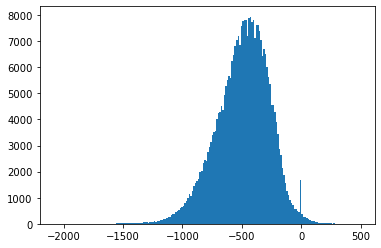
\includegraphics[width=0.3\linewidth]{images/rec_100_hist_measurements_200_bins.png}}
\hfill
\subfloat[Record 102]{%
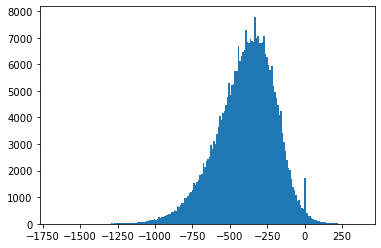
\includegraphics[width=0.3\linewidth]{images/rec_102_hist_measurements_200_bins.png}}
\hfill
\subfloat[Record 115]{%
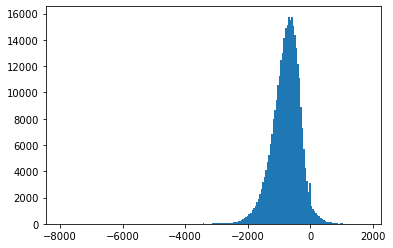
\includegraphics[width=0.3\linewidth]{images/rec_115_hist_measurements_200_bins.png}}
\\
\subfloat[Record 202]{%
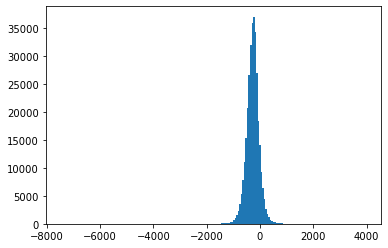
\includegraphics[width=0.3\linewidth]{images/rec_202_hist_measurements_200_bins.png}}
\hfill
\subfloat[Record 208]{%
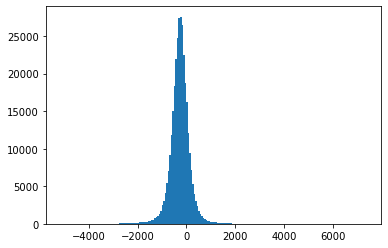
\includegraphics[width=0.3\linewidth]{images/rec_208_hist_measurements_200_bins.png}}
\hfill
\subfloat[Record 234]{%
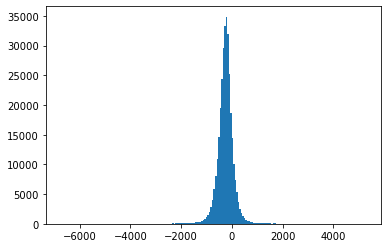
\includegraphics[width=0.3\linewidth]{images/rec_234_hist_measurements_200_bins.png}}
\caption{Histograms of measurement values with the sparse binary sensing matrix
with $m=256,n=512,d=4$ in 200 bins}
\label{fig-cs-codec:y:hist:200}
\end{figure}


\subsection{Quantization Parameter}

\begin{figure*}
\centering
\subfloat[$q$ vs $\prd$]{%
\includegraphics[width=0.32\linewidth]{images/rec_100_q_vs_prd_at_mr.pdf}}
\hfill
\subfloat[$q$ vs $\pss$]{%
\includegraphics[width=0.32\linewidth]{images/rec_100_q_vs_pss_at_mr.pdf}}
\hfill
\subfloat[$\pms$ vs $\pss$]{%
\includegraphics[width=0.32\linewidth]{images/rec_100_pms_vs_pss_at_q.pdf}}
\hfill
\caption{Variation of compression statistics vs quantization parameter
at different measurement ratios $\frac{m}{n}$
for record 100}
\label{fig-cs-codec-100-q-mr-stats}
\end{figure*}


The quantization step is a key contributor to compression
savings. This can be studied better under the fixed
quantization mode. In the first experiment, we compress
the data from record 100 at different values of
the quantization parameter $q$ and PMS.
The results are shown in \cref{fig-cs-codec-100-q-mr-stats}.
The number of measurements ($m$) has been chosen to vary from
$20\%$ to $60\%$ of the window size ($n$).
$q$ varies from $0$ to $7$.
(a) shows that reconstruction quality doesn't
change much from $q=0$ till $q=4$ after which it starts degrading.
As expected, the PRD degrades as $m$ is reduced.
(b) shows that PSS (percentage space saving) increases linearly
with $q$. As $q$ increases, the size of the alphabet for
entropy coding reduces and this leads to increased space savings.
(c) shows the variation of PSS with PMS at different values of $q$.
PSS increases linearly with PMS. Also, PSS is much higher
than PMS at higher quantization levels.

Increasing quantization linearly increases the PSS.
Since up to $q=4$, there is no noticeable
impact on PRD, as seen in panel (a), it is safe
to enjoy these savings in bit rate. 
At $40\%$ PMS, one can attain up to $69.3\%$ PSS without
losing any reconstruction quality.

\Cref{fig:100:q:0-7} shows the impact of the
quantization step on the reconstruction quality
for a small segment of record 100.
The first panel shows the original (digital) signal.
The remaining panels show the reconstruction at different $q$ values
using the BSBL-BO algorithm.
The reconstruction visual quality is excellent
up to $q=5$ (PRD below 7\%), good at $q=6$ (PRD at 9\%)
and clinically unacceptable at $q=7$
(with PRD more than 15\%).
One can see significant waveform distortions at $q=7$.
Also, note how the quality score keeps increasing till
$q=4$ and starts decreasing after that with a massive
drop at $q=7$.

\begin{figure}
\centering 
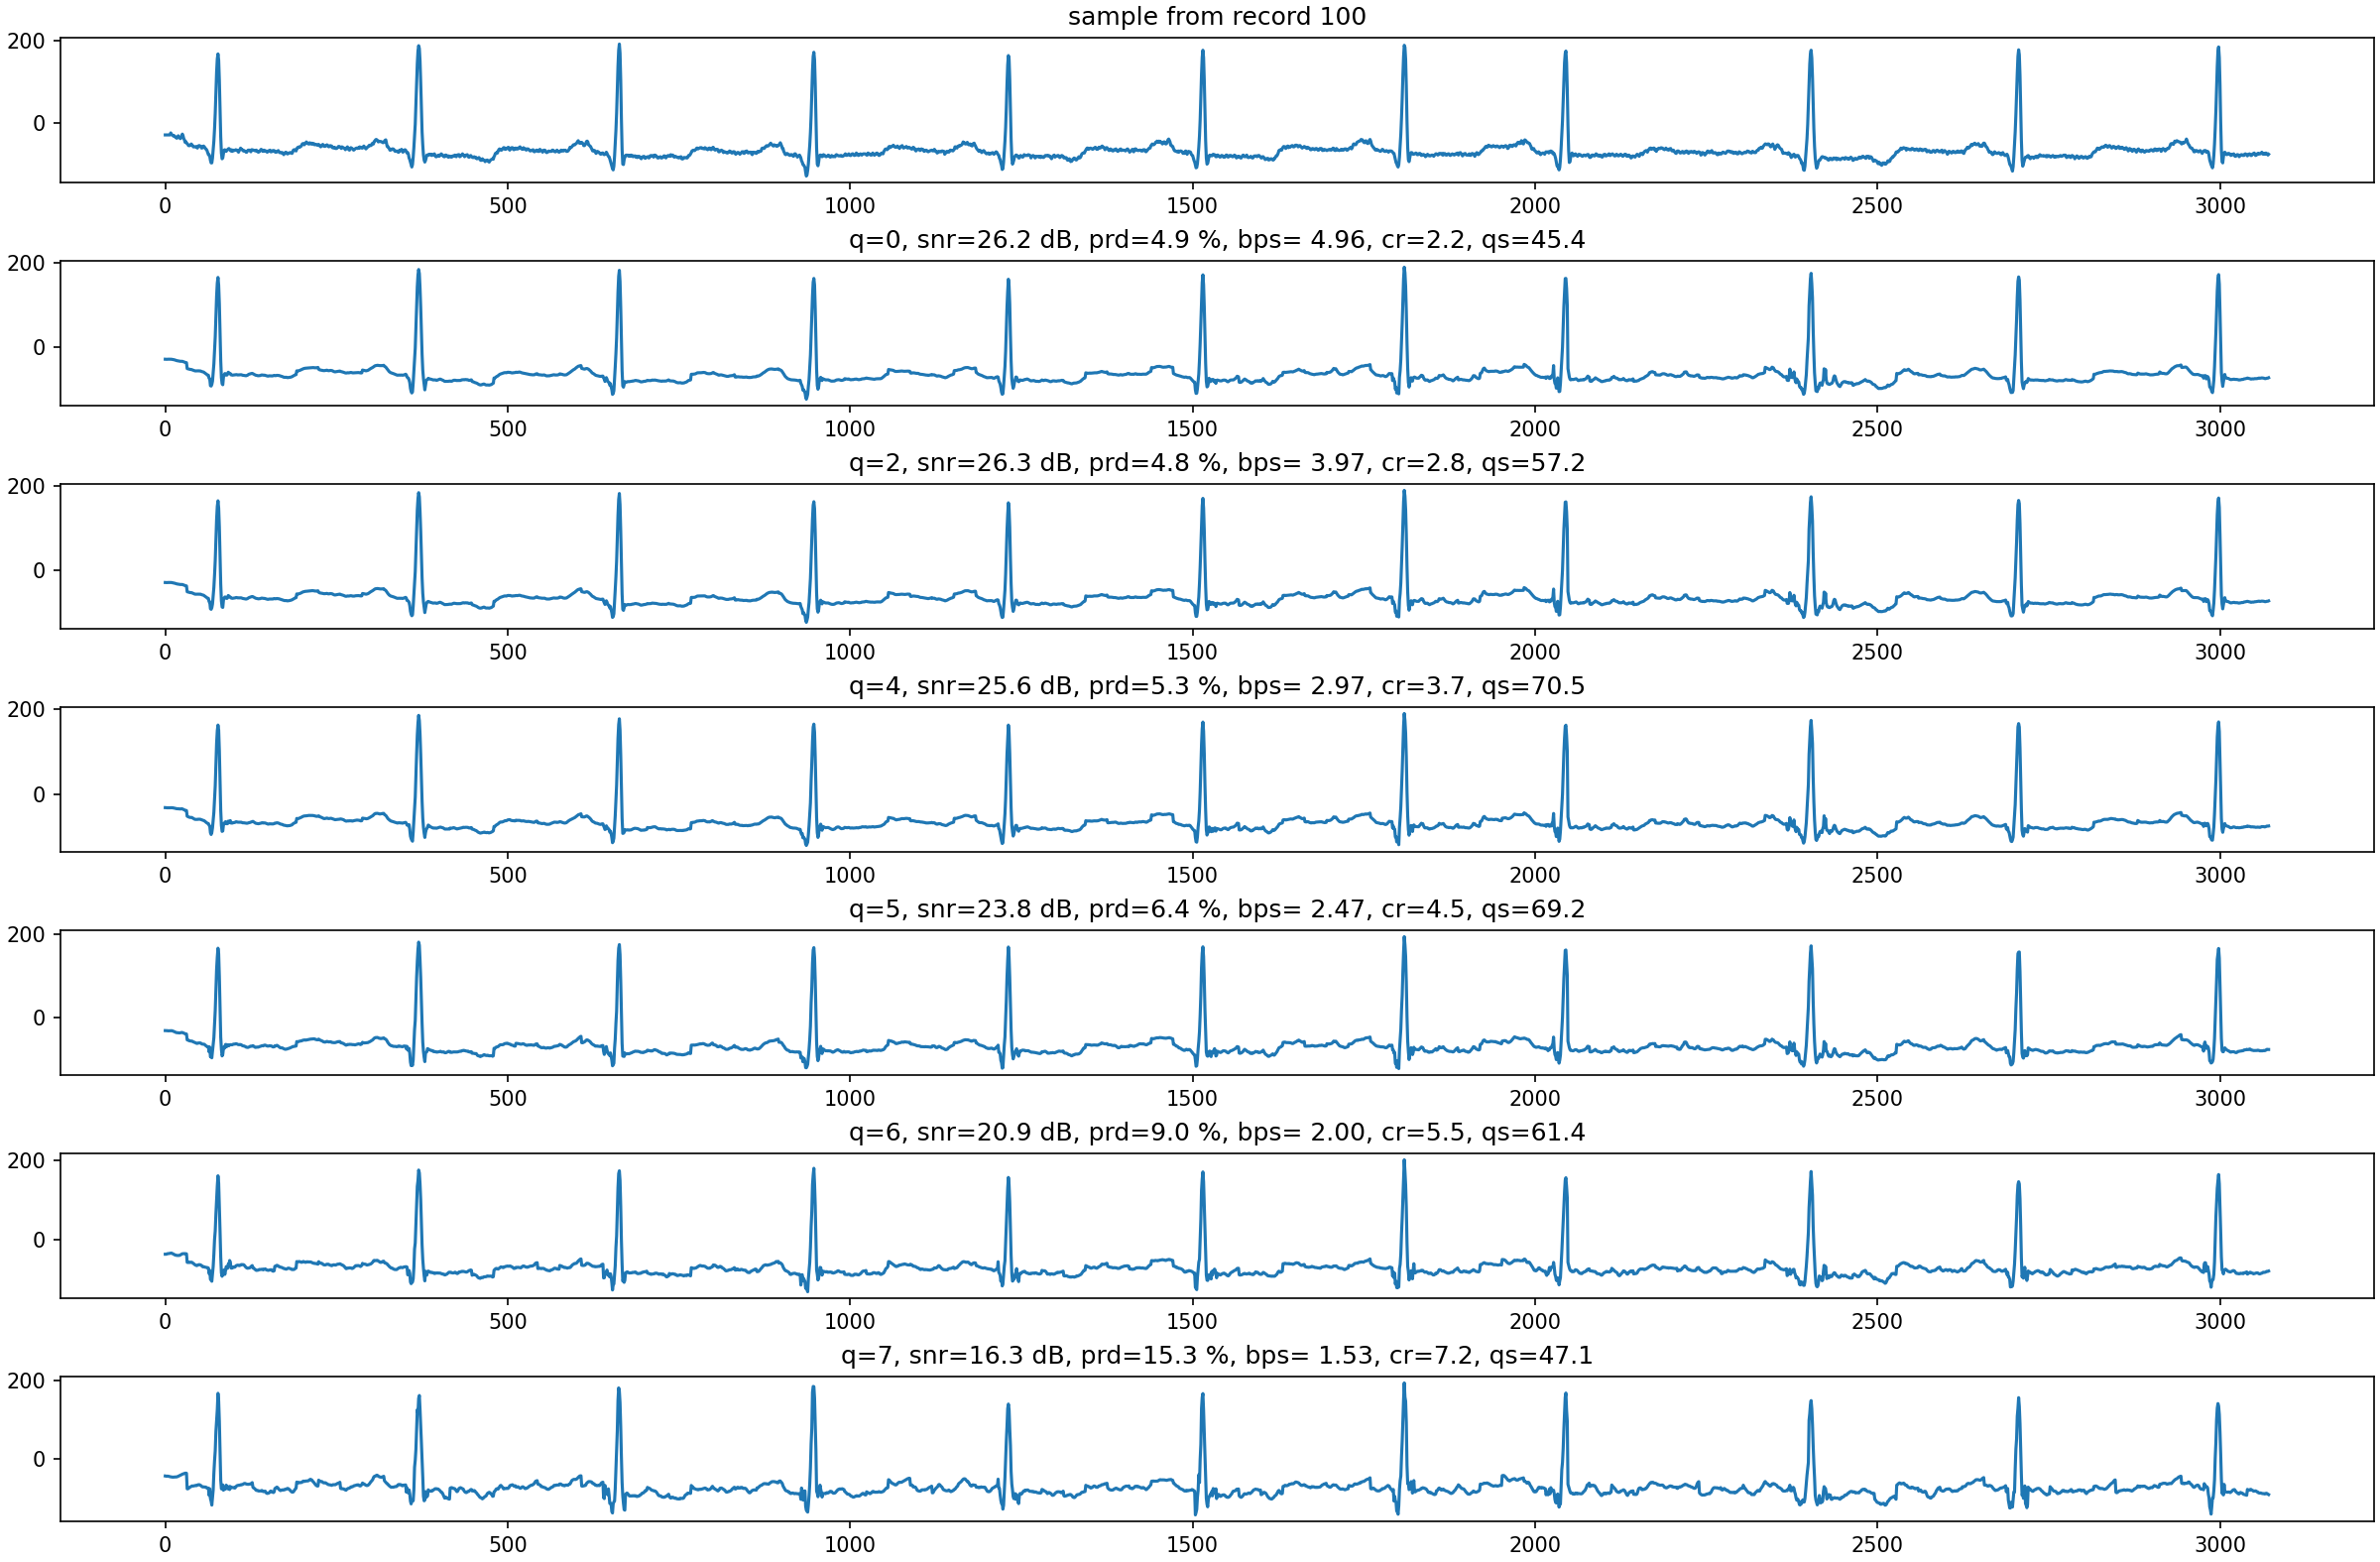
\includegraphics[width=0.95\linewidth]
{images/rec_100_q_cr_prd_qs.png}
\caption{Reconstruction of a small segment of record 100
for different values of $q=0,2,4,5,6,7$ with $m=256,n=512,d=4$
under non-adaptive quantization.
The block size for the BSBL-BO decoder is $32$.}
\label{fig:100:q:0-7}
\end{figure}
In the remaining experiments, we will be using adaptive
quantization.

We note that Mamaghanian et al. \cite{mamaghanian2011compressed}
have used an inter-packet redundancy removal step before
Huffman coding. They suggest that measurements of consecutive
windows are correlated due to the periodic nature of the ECG signal.
However, we suspect that this was happening due to the use of
unsigned digital values with a large DC component in their design.
Since we removed the baseline from the signal before compression,
we didn't notice any significant inter-packet redundancy.
Hence, we haven't included any redundancy removal block in our encoder.

\subsection{Space Savings}

In this experiment, we report the variation of
the percentage space savings ($\pss$)
with the percentage measurement savings ($\pms$)
under different encoder configurations.
We chose the window size $n=512$.
PMS varies from $20\%$ to $80\%$.
Correspondingly $m$ varies from $410$ down to $77$.
For each choice of $m$ and $n$, we constructed
binary sensing matrices $\Phi$
for two different values of $d$ at $d=4$ and $d=12$.
All 48 records were encoded and $\pss$ was measured
separately for each of them.
\Cref{fig-res-pms-pss-errorbar} shows the variation
of mean $\pss$ (over records) with $\pms$ along with
error bars for standard deviation across records
at each $\pms$.
We note that $d=12$ gives slightly better compression.
However, the difference is not significant and it decreases
as PMS increases. The small error bars indicate that the
compression ratio doesn't vary much from record to record.
At low PMS, we can see that the compression scheme can
give additional savings of up to 25\%. The trend line
is linear and savings reduce linearly to 5\% at 85\% PMS.

\begin{figure}
\centering
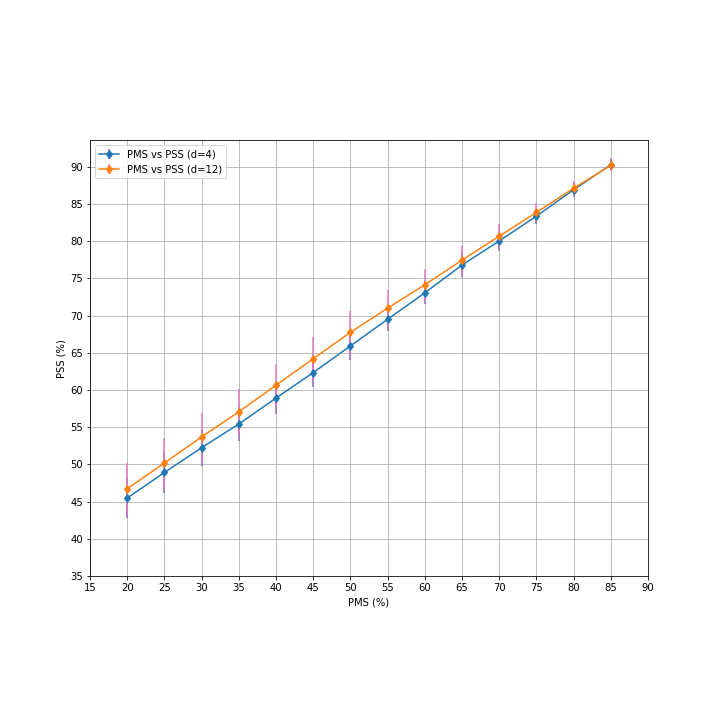
\includegraphics[width=0.95\linewidth]{images/bsbl/pms-vs-pss-errorbar.png}
\caption{Error bars for variation of mean $\pss$
with $\pms$ for 48 records at $d=4$ and $d=12$.}
\label{fig-res-pms-pss-errorbar}
\end{figure}

\Cref{fig-res-pms-pss-boxplot-d4} shows more detailed box plots
of variation of PMS across the 48 records at different PMS values.

\begin{figure}
\centering
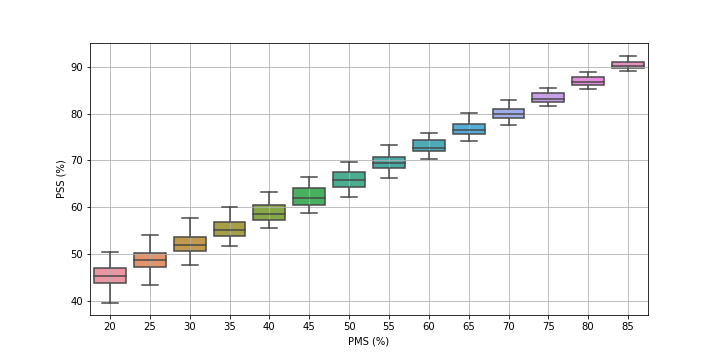
\includegraphics[width=0.95\linewidth]{images/bsbl/pms-vs-pss-boxplot-d4.png}
\caption{PMS vs PSS box plots over 48 records at $d=4$}
\label{fig-res-pms-pss-boxplot-d4}
\end{figure}
In the following, we will report results for $d=4$
configuration. Results are similar for $d=12$.

We measured the overhead of bits required to
encode the stream and frame headers. The overhead
varies from 0.07\% at PMS=20\% to about 0.4\% at PMS=80\%
on average. At higher PMS there are very few measurements
to encode. Hence overhead is higher. Increasing the frame
size will reduce the overhead. However, this will cause
delays in a real-time system since a frame cannot be decoded
till its full payload has been received. 

The bits per sample vary from
$6 \pm 0.3$ $\bps$ at PMS=20\% down to
$1 \pm 0.1$ $\bps$ at PMS=85\%.
This is significant compared to the uncompressed
rate of $11$ bits per sample.

Savings gain can be measured as the difference $\pss - \pms$.
\Cref{fig-res-pms-gain-boxplot-d4} shows the box plots of
savings gains at different PMS levels.
Savings gain varies from $25\pm3\%$ at PMS=20\% down to
$5.3 \pm 0.9\%$ at PMS=85\%. More measurements lead to
more savings via the quantization, clipping and entropy coding steps.


\begin{figure}
\centering
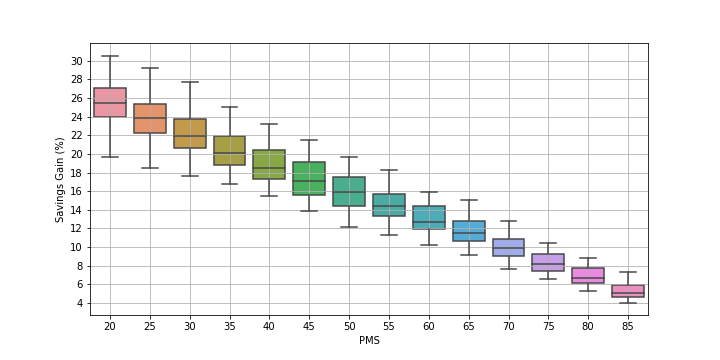
\includegraphics[width=0.95\linewidth]{images/bsbl/pms-vs-saving-gain-boxplot.png}
\caption{PMS vs Savings gain (PSS - PMS) box plots over 48 records at $d=4$}
\label{fig-res-pms-gain-boxplot-d4}
\end{figure}

Our adaptive quantization scheme is designed to
keep the noise introduced by quantization and clipping
steps to reasonable levels.
\Cref{fig-res-pms-q-snr-boxplot-d4} shows the box plots
of variation of quantization noise SNR across the 48
records at different PMS. It is clear that quantization
SNR remains limited between 35 and 40 dB.

\begin{figure}
\centering
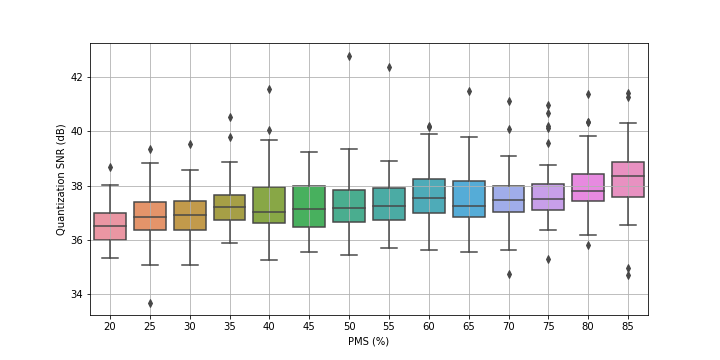
\includegraphics[width=0.95\linewidth]{images/bsbl/pms-vs-q-snr-boxplot-d4.png}
\caption{PMS vs Quantization SNR box plots over 48 records at $d=4$}
\label{fig-res-pms-q-snr-boxplot-d4}
\end{figure}

Compression is to no avail if the signal cannot be reconstructed
faithfully. The reconstruction heavily depends
on the choice of the sparse recovery algorithm.
In the following, we present our results for two different sparse
recovery approaches.

\subsection{Reconstruction with BSBL-BO}

\Cref{fig-res-bsbl-pms-prd-errorbar} shows the variation
of mean PRD with PMS for $d=4$ as well as $d=12$ when BSBL-BO
reconstruction algorithm is used in the decoder. The error
bars show the standard deviation of PRD across the 48 records.
We have drawn additional lines for 2\% and 9\% PRD that indicate
very good and good reconstruction levels. 
Surprisingly, $d=4$ gives us better PRD. 
We can see that mean PRD is below 9\% level till up to 65\% PMS.
At this PMS, we have a PSS of about 77\% (\cref{fig-res-pms-pss-errorbar}).

\begin{figure}
\centering
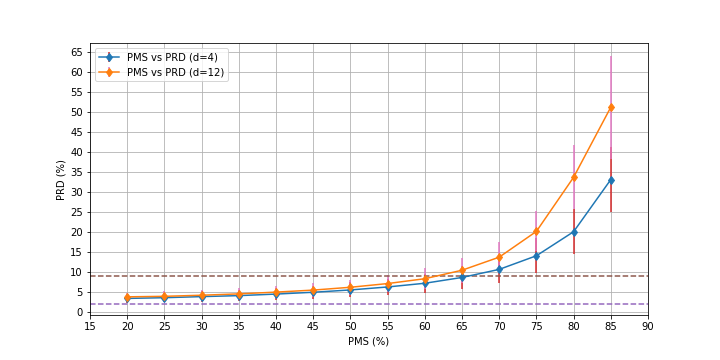
\includegraphics[width=0.95\linewidth]{images/bsbl/pms-vs-prd-errorbar.png}
\caption{Error bars for variation of PMS vs mean PRD at $d=4$ and $d=12$
for reconstruction with the BSBL-BO algorithm.}
\label{fig-res-bsbl-pms-prd-errorbar}
\end{figure}


% \begin{figure}
% \centering
% 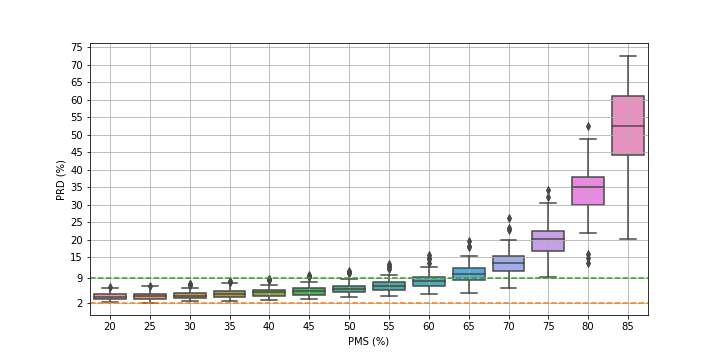
\includegraphics[width=0.95\linewidth]{images/bsbl/pms-vs-prd-boxplot-d12.png}
% \caption{PMS vs PRD box plots over 48 records at $d=12$ for reconstruction
% with the BSBL-BO algorithm.}
% \label{fig-res-bsbl-pms-prd-boxplot-d12}
% \end{figure}

\Cref{fig-res-bsbl-pms-prd-boxplot-d4} provides more detailed box plots
for the variation of PRD with PMS across the 48 records at $d=4$.
\begin{figure}[!t]
\centering
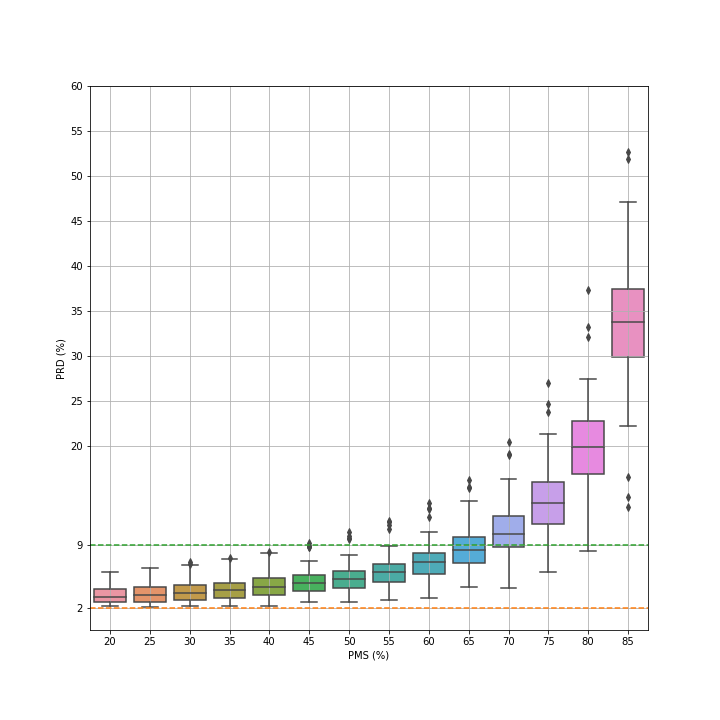
\includegraphics[width=0.95\linewidth]{images/bsbl/pms-vs-prd-boxplot-d4.png}
\caption{PMS vs PRD box plots over 48 records at $d=4$ for reconstruction
with BSBL-BO algorithm}
\label{fig-res-bsbl-pms-prd-boxplot-d4}
\end{figure}

\subsection{Reconstruction with CS-NET}
For CS-NET, a window size of $n=256$ was chosen.

\Cref{fig-res-csnet-pms-prd-errorbar} shows the variation
of mean PRD with PMS for $d=4$ when CS-NET is used in the decoder.
\Cref{fig-res-csnet-pms-prd-boxplot}  more detailed box plots
for the variation of PRD with PMS across the 48 records.
We note that CS-NET can reconstruct well up to 80\% PMS
with 7\% additional space savings.

\begin{figure}
\centering
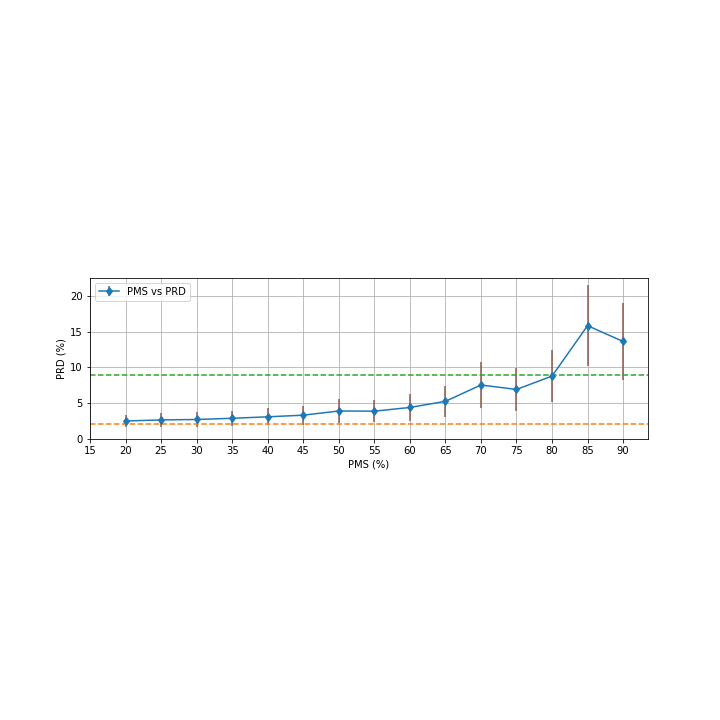
\includegraphics[width=0.95\linewidth]{images/csnet/pms-vs-prd-errorbar.png}
\caption{Error bars for variation of mean PRD with PMS at $d=4$ for reconstruction with
CS-NET.}
\label{fig-res-csnet-pms-prd-errorbar}
\end{figure}

\begin{figure}
\centering
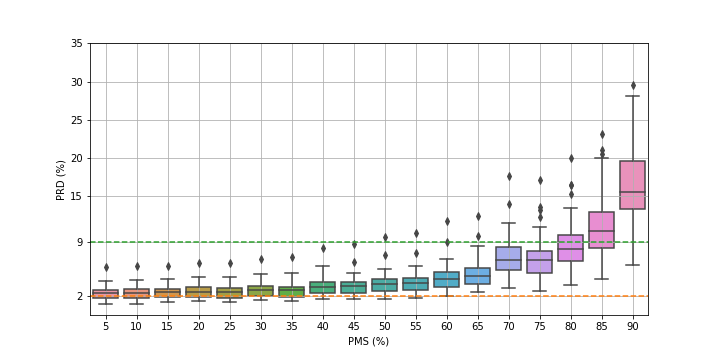
\includegraphics[width=0.95\linewidth]{images/csnet/pms-vs-prd-boxplot.png}
\caption{PMS vs PRD box plots over 48 records at $d=4$ for reconstruction
with CS-NET}
\label{fig-res-csnet-pms-prd-boxplot}
\end{figure}


\subsection{Comparison}
Zhang et al. \cite{zhang2021csnet} have reported
optimal PMS values for different methods (BP, OMP, BSBL-BO, CSNet, etc.)
for PRD=9\% for a subset of test records for $n=256$.
In their setup, $\Phi$ is RIP satisfying matrix which is different
from the binary sensing matrix used in our setup.
For BSBL-BO reconstruction,
we report the needed PMS as well as the corresponding PSS
for these records for a $\prd \leq 9 \%$.
in \cref{tbl-bsbl-optimal-pss-prd}.
While our codec requires slightly more measurements
due to the sparsity of the sensing matrix, it consistently
outperforms in compression due to additional space
savings from quantization and entropy coding.

\begin{table}[ht]
\centering
\caption{Required PMS and corresponding PSS for BSBL-BO for
a target PRD $\leq 9\%$}
\begin{tabular}{ccccc}
\toprule
Record & Ref PMS & Our PMS & PSS & PRD\\
\midrule 
100 & 71 & 65 & 77.2 & 8.3 \\  
101 & 71 & 65 & 76.5 & 8.5 \\  
102 & 70 & 61 & 75.6 & 8.5 \\  
107 & 74 & 64 & 74.4 & 8.5 \\  
109 & 75 & 70 & 78.8 & 8.7 \\  
111 & 69 & 63 & 74.5 & 8.6 \\
115 & 68 & 66 & 78 & 8.5 \\  
117 & 74 & 72 & 83.8 & 6.5 \\  
118 & 76 & 68 & 81 & 8.5 \\  
119 & 71 & 69 & 81.3 & 8.3 \\
\bottomrule
\end{tabular}
\label{tbl-bsbl-optimal-pss-prd}
\end{table}


Mamaghanian et al. \cite{mamaghanian2011compressed}
report their best result for CS for record 107
for which they report that "good" ($\prd \leq 9\%$)
signal recovery can be achieved up to a PSS of 74\%.
For our codec with BSBL-BO reconstruction, good
recovery was achieved up to a PSS of 75 \%.

% %!TEX root = paper_ecg_cs_codec.tex
\section{Conclusion}
\label{sec:conclusion}

The key contributions of our encoder architecture are the following:

\begin{itemize}
    \item We have presented a digital compressive sensing-based encoder
    design including adaptive digital quantization
    and entropy coding which can be
    implemented entirely using integer arithmetic.
    \item We have demonstrated that ANS-based arithmetic coding can
    lead to significant space savings.
    \item We have demonstrated that we don't need a hard-coded
    code-book for entropy coding. We can simply model the
    measurement values distributed as quantized Gaussian values
    for effective entropy coding.
    \item We use simple mean and standard deviation as the entropy model
    parameters which can be dynamically adapted. The overhead of
    the side information is negligible.
    \item We have demonstrated up to $16\%$ of additional space
    savings contributed by the quantization and entropy coding steps.
    \item We have described a complete bitstream specification for
    the carriage of all the side information needed to decode the
    entropy-coded compressive measurements.
\end{itemize}

The software code implementing this codec
and all scripts for the experimental studies conducted
in this work have been released as opensource software
on GitHub \cite{kumar2022ecgcodec}.



% \input{sec_tables}
\appendix
%!TEX root = paper_ecg_cs_codec.tex
\section{Compressive Sensing}
\label{appsec:cs}
Under the digital CS paradigm, we assume that the
signals have passed through the analog to digital
converter (ADC) and are represented using signed integers
at a specific resolution.

CS is an emerging signal compression paradigm that relies
on the sparsity of signals (in an appropriate basis)
to compress using incoherent measurements.
The basic model can be expressed as:
\begin{equation}
\by = \Phi \bx + \be
\end{equation}
where $\bx \in \RR^n$ is a signal to compress
(of length $n$). $\Phi \in \RR^{m \times n}$
is a sensing matrix that compresses $\bx$
via linear measurements. Each row of $\Phi$
represents one linear measurement as a linear
functional on $\bx$. $\by$ is a measurement
vector consisting of $m$ distinct measurements
done on $\bx$. By design $\Phi$ is a full
rank matrix. Hence every set of $m$ columns of $\Phi$
is linearly independent. $\be \in \RR^m$ is the
error/noise introduced during the measurement process.
In our digital CS paradigm, the noise is introduced
by the quantization step in our encoder.
In our case, $\bx$ is a window of a raw ECG record
from one channel/lead. 
Often $\bx$ is not sparse by itself but is sparse
in some orthonormal basis $\Psi$ expressed as
$\bx = \Phi \alpha$ and the representation $\alpha$
is sparse. ECG signals exhibit sparsity in wavelet
bases.

Most natural signals have richer structures beyond
sparsity. A common structure is natural signals
is a block/group structure \cite{eldar2010block}. 
We introduce the block/group structure on $\bx$ as
\begin{equation}
\bx = \begin{pmatrix}
\bx_1 & \bx_2 & \dots & \bx_g
\end{pmatrix}
\end{equation}
where each $\bx_i$ is a block of $b$ values.
The signal $\bx$ consists of $g$ such blocks/groups.
Under the block sparsity model, only a few $k \ll g$
blocks are nonzero (active) in the signal $\bx$
however, the locations of these blocks are unknown.
We can rewrite the sensing equation as:
\begin{equation}
\by = \sum_{i=1}^g \Phi_i \bx_i + \be
\end{equation}
by splitting the sensing matrix into blocks of columns appropriately.

\subsection{Block Sparse Bayesian Learning}
Under the sparse Bayesian framework, each block
is assumed to satisfy a parametrized multivariate
Gaussian distribution:
\begin{equation}
\PP(\bx_i ; \gamma_i, \bB_i) = \NNN(\bzero, \gamma_i \bB_i), \Forall i=1,\dots,g.
\end{equation}
The covariance matrix $\bB_i$ captures the intra block correlations.
We further assume that the blocks are mutually uncorrelated.
The prior of $\bx$ can then be written as
\begin{equation}
\PP(\bx; \{ \gamma_i, \bB_i\}_i ) = \NNN(\bzero, \Sigma_0)
\end{equation}
where
\begin{equation}
\Sigma_0 = \text{diag}\{\gamma_1 \bB_1, \dots, \gamma_g \bB_g \}.
\end{equation}
We also model the correlation among the values
within each active block as an AR-1 process.
Under this assumption the matrices
$\bB_i$ take the form of a Toeplitz matrix
\begin{equation}
\bB = \begin{bmatrix}
1 & r & \dots & r^{b-1}\\
r & 1 & \dots & r^{b-2}\\
\vdots &  & \ddots & \vdots\\
r^{b-1} & r^{b-2} & \dots & 1
\end{bmatrix}
\end{equation}
where $r$ is the AR-1 model coefficient.
This constraint significantly reduces the model parameters to be learned.

Measurement error is modeled as independent zero-mean Gaussian
noise $\PP(\be; \lambda) \sim \NNN(\bzero, \lambda \bI)$.
BSBL doesn't require us to provide the value of noise variance
as input.
It is able to estimate $\lambda$ within a algorithm.

The estimate of $\bx$ under Bayesian learning framework
is given by the posterior mean of $\bx$ given the measurements $\by$.



\section{Entropy Coding}
\label{appsec:ec}
From the perspective of entropy coding, a \emph{symbol}
is a unit of information to be transmitted. For us,
each value in a measurement vector is a symbol.
An \emph{alphabet} is the set of all symbols that
can be transmitted. For us, it is the set of integral
values that the entries in a measurement vector can take.
A \emph{message} is a sequence of symbols to be transmitted.
For us, it is the sequence of all measurement values.
There are two primary types of coding schemes: symbol
codes and stream codes. A symbol code (e.g., Huffman code)
assigns a unique bit string to each symbol.
A stream code maps a message (a sequence of symbols)
to a (large) integer. Symbol codes approach optimal
compression only when the Shannon information content
of each symbol happens to be close to powers of $2$.
In particular, Huffman coding is not optimal
since it encodes each symbol using an integral
number of bits. It is not capable of encoding symbols using
fractional number of bits.

In contrast, stream codes can achieve near-optimal
compression for any probability distribution.
Arithmetic Coding (AC) \cite{rissanen1979arithmetic,witten1987arithmetic}
encodes the entire message of symbols into a single (large) integer
enabling fractional bits for different symbols in a message.
A recent family of entropy coders called Asymmetric Numeral Systems (ANS)
\cite{duda2013asymmetric}
allows for faster implementation
thanks to directly operating
on a single natural number representing the current information.
It combines the speed of Huffman coding with compression rate
of arithmetic coding.
The \emph{constriction} library \cite{bamler2022constriction} provides
a nice way to model each symbol in a message as a sample from
a given probability distribution and then encode it using ANS.

% \subsection{Asymmetric Numeral Systems}





% Can use something like this to put references on a page
% by themselves when using endfloat and the captionsoff option.
\ifCLASSOPTIONcaptionsoff
  \newpage
\fi


\bibliographystyle{IEEEtran}
% argument is your BibTeX string definitions and bibliography database(s)
\bibliography{IEEEabrv,references}

% that's all folks
\end{document}

